% !TEX root = main.tex
\documentclass[12pt, letterpaper]{article} % Choose article, report, or book class

% --- Preamble ---
\usepackage[utf8]{inputenc}       % For Unicode characters
\usepackage{amsmath, amssymb}     % Math symbols
\usepackage{graphicx}           % Include images
\usepackage{geometry}           % Adjust margins
\usepackage{hyperref}             % Create clickable links
\usepackage{natbib}             % For citation management
\usepackage{xcolor}             % For color options
\usepackage{float}              % For precise figure placement
\usepackage{lipsum}             % For dummy text (remove in final document)
\usepackage{setspace}         %For setting line spacing (e.g., double spacing)

% --- Customization ---
\geometry{a4paper, margin=1in}   % Set page margins
\hypersetup{colorlinks=true,   % Color links instead of boxes
            linkcolor=blue,
            citecolor=blue,
            urlcolor=blue}

\title{A Comprehensive Literature Review on [LLMs For Mental Health Therapeutics]}
\author{
  Roop Kumar \and
  Thi Thuy Dung Tran\and
  Chatdanai Pangwisate \and
  Kasey Kelly \and
  Naga Sowjanya Barla
}

\date{}
\usepackage{natbib}
\usepackage{hyperref} % Highly recommended for clickable citations

% --- Begin Document ---
\begin{document}

\maketitle  % Display title, author, and date

\begin{abstract}
    This study presents a comprehensive review of the capabilities, limitations, and ethical implications of using large language models (LLMs) in mental health therapeutics. We explore the evolution of LLMs, from early models like ELIZA to modern architectures such as GPT-4 and FLAN-T5, and evaluate their effectiveness across mental health prediction and support tasks including stress, depression and suicide risk detection. Drawing on fine-tuning strategies, zero- and few-shot prompting and instruction learning, the study analyzes how models such as Alpaca, FLAN-T5 and GPT variants perform using benchmark datasets like Reddit Suicide Watch and EmpatheticDialogues. We highlight the trade-offs between general-purpose and fine-tuned models in accuracy, empathy, and real-time responsiveness. Special focus is given to the privacy, ethical and safety risks inherent in deploying AI chatbots in clinical settings. The study concludes with actionable recommendations for prompt engineering, dataset curation, personalization and crisis response safeguards to improve the reliability of LLMs for mental health applications. % Include the content of abstract.tex
\end{abstract}

\tableofcontents 
\section{Introduction}
    Mental health is a critical component of public health, with profound implications for individuals and societies worldwide. According to the U.S. National Institute of Mental Health (NIMH), 22.8 percent of U.S. adults experienced mental illness in 2021, while the World Health Organization (WHO) reports that mental health disorders account for 30 percent of the global non-fatal disease burden, making them a leading cause of disability. These statistics highlight the urgent need for innovative solutions to address the growing mental health crisis, particularly in light of the global shortage of mental health professionals.

Large Language Models (LLMs) represent a groundbreaking advancement in artificial intelligence, characterized by their ability to process and generate human-like text at an unprecedented scale. Built on sophisticated architectures such as the Transformer, these models have demonstrated remarkable capabilities in understanding context, generating coherent responses, and performing complex language tasks. The evolution of LLMs, from early statistical models to modern systems like GPT-4 and LLaMA, has been driven by innovations in model architecture, training techniques, and computational efficiency.

The Transformer architecture, introduced by Vaswani et al. (2017), serves as the foundation for most contemporary LLMs. Its key innovation—the self-attention mechanism—enables models to dynamically weigh the importance of different words in a sequence, overcoming the limitations of earlier recurrent neural networks (RNNs) and long short-term memory (LSTM) models. Unlike RNNs, which process text sequentially and struggle with long-range dependencies, Transformers parallelize computations and capture global context more effectively. This architectural superiority has led to significant improvements in tasks requiring nuanced language understanding, such as sentiment analysis, dialogue generation, and mental health support applications.

This study aims to address this gap by providing the first detailed review of LLM applications in mental health care with four key areas:

1. Datasets, models, and training techniques used in mental health applications.

2. Applications and conditions targeted by LLMs, along with validation measures.

3. Discrepancies between current tools and their practical implementation in clinical settings.

4. Ethical and privacy considerations surrounding the use of LLMs in sensitive mental health contexts.

\section{History of LLMs}
    \documentclass{article}
\usepackage{lipsum}

\subsection{Subtopic 1.1}

Einstein introduced the theory of relativity in 1905 \cite{arriba2024}.

\subsection{Subtopic 1.2}
\lipsum[5-6] 

\section{Privacy Concerns}
    \documentclass{article}
\usepackage{natbib}

... Some text ... \cite{gbollie2023}.  More text... \citep{sejnowski2023}
\dots

\bibliographystyle{apalike}
\bibliography{references} 

\section{Efficacy of Mental Health Chat Bots}
    Recent advancements in large language models (LLMs) have opened up more relevance in the field of digital mental health, offering scalable solutions for early detection, diagnosis and support. 
But the efficacy of the models is a very important consideration. 
 
This section explores the data sources, fine-tuning methods, performance trade-offs, and ethical implications of using AI-driven chatbots in mental health contexts. We highlight the impact of training data biases, discuss the balance between speed and accuracy and examine real-world risks including misinformation, user trust and demographic disparities.

\section{Model Training and Evaluation of LLMs in Mental Health}

\subsection{Model Training and Biases}

Chatbots and AI models designed for mental health support are predominantly trained on datasets derived from social media platforms, psychotherapy transcripts, and electronic health records (EHRs). A majority of models in the literature have been fine-tuned specifically for mental health prediction tasks using benchmark datasets such as \textit{Dreaddit}, \textit{DepSeverity}, \textit{SDCNL}, and \textit{CSSRS-Suicide} \cite{arriba2024}. These datasets are often annotated by human experts and sourced primarily from Reddit, enabling models to perform tasks such as binary stress classification, depression detection, and suicide risk estimation. While these data sources provide scalability, they also introduce significant demographic and cultural biases.

Bias remains a persistent challenge. Studies have highlighted how the overreliance on Reddit-based data skews model generalizability, often failing to capture the nuances of underrepresented groups \cite{li2023, gbollie2023}. Diagnostic models trained on such datasets may inadvertently reinforce users’ distress rather than challenge cognitive distortions, potentially increasing false positives. Furthermore, a lack of diversity in training data has led to measurable racial and gender biases in chatbot responses \cite{arriba2024}. Even expert-annotated corpora are susceptible to embedded stereotypes and confirmation bias, raising concerns about the validity of ground-truth labels \cite{greco2023}.

\subsection{Trade-Offs in Performance and Design}

Performance trade-offs are evident across model size, inference method, and processing strategy. Larger general-purpose models such as GPT-4 and FLAN-T5 offer faster response times, while smaller fine-tuned models like Mental-Alpaca often achieve higher task-specific accuracy \cite{xu2024}. Improved prompt engineering can enhance inference speed, but often at the cost of response quality. Stream-processing models allow for real-time interaction but demand continuous updating, whereas batch-processing models deliver greater accuracy by processing data in aggregate — albeit with delayed outputs \cite{mcgorry2025}.

Fine-tuning strategies play a central role in improving performance. Approaches such as instruction tuning and LoRA (Low-Rank Adaptation) have been applied to enhance LLMs for cognitive behavioral therapy (CBT) tasks. These models optimize predictions using cross-entropy loss, reducing divergence from human-labeled data \cite{na2024}.

\subsection{Accuracy, Coherence, and Logical Structure}

Transformer-based models have shown high accuracy in mental health tasks — with some detecting depression at rates exceeding 96\%, and chatbot-based models for cognitive impairment reaching over 80\% accuracy and 85\% recall \cite{greco2023, mcgorry2025}. Fine-tuned models such as Mental-FLAN-T5 consistently outperform zero-shot models like GPT-4 by up to 4.8\% in balanced accuracy \cite{xu2024}. However, zero-shot performance remains inconsistent, often fluctuating between 50\% and 83\% based on prompt structure.

In terms of coherence, rule-based conversational agents like Woebot and Wysa tend to outperform generative models in logical consistency and structure \cite{stade2024}. While GPT-4 responses are generally fluent, they can be overly generic and lack context-specific insight. In contrast, fine-tuned models offer more domain-relevant outputs. Notably, GPT-based models are sensitive to prompt phrasing, leading to variability in output quality and occasional overgeneralization — particularly in nuanced cases such as suicide risk \cite{sejnowski2023}.

\subsection{Risk of Misinformation and Ethical Implications}

Numerous studies caution against the misuse of LLMs in high-stakes contexts. Despite their sophistication, generative models are prone to producing “falsely reasonable” yet incorrect outputs. This poses a significant risk in mental health settings, where the consequences of misinformation can be severe. The absence of robust, systematic evaluation frameworks for mental health reasoning further compounds the issue \cite{greco2023}. In addition, the use of sensitive training data raises major concerns about privacy, consent, and ethical safeguards \cite{arriba2024}.

The potential for discriminatory outputs is fairly high given the lack of fairness assessments across different subgroups of population. Vulnerable users, including those in crisis, are particularly susceptible to receiving inaccurate or even harmful advice.

\subsection{Real-Time Performance vs. Quality}

While real-time models like GPT-4 excel in responsiveness, fine-tuned models such as Mental-FLAN-T5 yield more accurate and context-sensitive results with lower computational demands \cite{xu2024}. Enhancing model accuracy through prompt engineering often increases processing time. However, instruction-fine-tuned models manage to balance inference speed with depth of response more efficiently than zero-shot systems.

\subsection{Handling Ambiguity in User Prompts}

Fine-tuned models have demonstrated superior contextual understanding of vague or ambiguous queries related to stress or depression. In contrast, zero-shot models frequently default to binary or overly simplified interpretations. Few-shot learning methods have shown to improve GPT-4’s performance by around 4.1\% on ambiguous mental health queries \cite{xu2024}, indicating the need for more adaptable model architectures in this space.

\subsection{User Willingness and Perceptions}

User receptivity remains high, with 81.1\% of university students reporting willingness to engage with mental health chatbots — though only 4\% have done so in practice \cite{gbollie2023}. Younger demographics (18–35) show higher adoption rates, while users in acute distress often prefer human counselors due to trust and safety concerns.

Preferences are influenced by multiple factors. Stigma around seeking therapy makes some users favour AI over traditional face-to-face approaches. Conversational AI models like GPT-4 are generally preferred due to flexible and natural interaction. Rule-based model responses can often be repeated due to a fixed response database. However, concerns around privacy, transparency, and the potential for AI-generated errors remain key barriers to adoption.

\subsection{Outlook and Efficacy}

Emerging models such as CBT-LLM exemplify domain-specific fine-tuning tailored for psychological support. Evaluations show that such models outperform generic LLMs in both fluency and therapeutic relevance \cite{na2024}. Despite their promise, several researchers question whether LLMs truly “understand” mental health concerns or merely reflect user input in plausible ways — a phenomenon likened to a “reverse Turing test” \cite{sejnowski2023}.

A broader body of research suggests that while LLMs may augment therapists and automate diagnostics, they are not yet reliable standalone tools. Studies have shown marked symptom improvement using chatbot interventions (Hedge’s g = 0.64 for depression and 0.7 for distress) \cite{stade2024}, but little impact on long-term psychological well-being. Lastly, transformer-based models like BERT continue to demonstrate high efficacy for mental health classification, though their success remains closely tied to data quality and fine-tuning depth \cite{greco2023, li2023}. 

\section{Prompt Engineering}
    Prompt engineering refers to the deliberate design and manipulation of the inputs provided to large language models (LLMs) in order to optimise performance across various tasks. The body of research reviewed below collectively highlights that the structure, clarity, and contextual richness of a prompt significantly affect an LLM’s ability to generalise, reason, and generate high-quality responses. A critical analysis of these studies reveals an evolving understanding of how prompt structure influences LLM outputs, not only in simple tasks but also in complex, reasoning-intensive scenarios, offering key implications for their use in sensitive applications such as mental health support.
\cite{garg2021transformers} examine the in-context learning capabilities of transformer-based models, focusing on their ability to perform simple functions like sorting and pattern recognition. Their findings underscore that prompt structure is particularly crucial for enabling generalisation in tasks that fall just beyond training data, what they call "medial" tasks. Notably, as task complexity increases, the model's performance degrades unless the prompt is structured to support more abstract reasoning. This introduces an important insight: while LLMs can simulate learning through prompt engineering, this ability is fragile and highly dependent on how well the prompt scaffolds the task \cite{garg2021transformers}.
\cite{brown2020language} extend this idea through the concept of few-shot learning, showing that providing clear, structured examples within prompts dramatically improves performance. They find that including multiple relevant task examples (as opposed to zero- or one-shot prompts) increases contextual understanding and reduces ambiguity. Together, these studies suggest that prompt engineering is not just about making inputs readable, it is about making the task learnable within the constraints of the LLM’s architecture (\cite{brown2020language}). This has direct implications for mental health chatbots, where ambiguous user input must be interpreted with nuance and sensitivity.
While Garg and Brown focus on prompt clarity and structure in general task completion, more recent work by \cite{wang2022self} and \cite{yao2023tree} pushes this further by exploring how prompting can shape the reasoning process of LLMs. \cite{wang2022self} Chain-of-Thought (CoT) prompting introduces intermediate reasoning steps that mimic human-like deliberation. Their results show that CoT prompting not only improves task performance but also maintains accuracy as task complexity increases, a contrast to \cite{garg2021transformers} finding that LLM performance diminishes under complexity. This suggests that introducing a structured reasoning process within prompts can compensate for limitations in generalisation, further supporting the need for more sophisticated prompt strategies (\cite{wang2022self}).
Building on this, \cite{yao2023tree} propose Tree-of-Thought (ToT) prompting, which enables the model to explore multiple solution paths before selecting the most appropriate one. Unlike CoT, which tends to follow a linear reasoning path, ToT encourages branching thought processes and reflective evaluation. This aligns with decision-making frameworks used in cognitive-behavioural therapy (CBT) and other mental health contexts, where multiple perspectives and reflective thinking are essential. The findings from ToT experiments demonstrate that LLMs can be prompted not just to answer questions, but to think through them in a structured, human-like way, critical for engaging users in therapeutic dialogue (\cite{yao2023tree}).
Further refining this approach, \cite{yao2022react} introduce ReAct prompting, which separates reasoning from action. Here, the model first reasons through the problem, then generates a final output. This division ensures that responses are not just reactive but deliberative, enhancing LLM performance in interactive tasks like question-answering. In the context of mental health, this separation is particularly important: it mirrors the therapeutic process of validating emotions before suggesting actions, a key to empathetic engagement (\cite{yao2022react}).
Taken together, these studies highlight a central inference: high-quality LLM outputs are not merely a function of the model’s size or training data, but of how intelligently they are prompted. While early research like that of \cite{garg2021transformers, brown2020language} emphasised prompt clarity and example inclusion, newer approaches like CoT, ToT, and ReAct show that prompting can simulate cognitive processes such as reflection, evaluation, and decision-making. This progression reflects a broader shift in prompt engineering, from focusing solely on inputs to shaping the model’s thinking process.
Implications for Mental Health Chatbots
These findings carry profound implications for the design of LLM-based mental health chatbots. Individuals in psychological distress often struggle to express themselves clearly or to provide structured input. This makes user-initiated prompt quality highly variable. If the chatbot relies solely on direct user input, its responses risk being generic, inappropriate, or even harmful.
To address this, the chatbot must act as an intermediary prompt engineer, restructuring, expanding, or interpreting user inputs using internal reasoning frameworks. Techniques such as CoT and ReAct can be embedded into the system to simulate deeper understanding, allowing the model to "think through" user concerns before responding (\cite{wang2022self, yao2022react}). For example, instead of responding directly to “I feel off,” the model could internally generate a series of interpretive questions, reflections, and emotional validations before offering a meaningful reply.
Additionally, the insights from ToT prompting can be used to generate multiple potential responses and select the one that best aligns with therapeutic goals, such as validation, reflection, or gentle guidance (\cite{yao2023tree}). In this way, the chatbot mimics the thoughtful deliberation of a trained therapist, increasing the likelihood of meaningful engagement.
Finally, prompt engineering becomes not just a tool for improving performance but a safeguard. By structuring internal reasoning processes, LLMs can avoid surface-level interpretations and respond in ways that are more aligned with therapeutic best practices, improving both the emotional and clinical efficacy of the chatbot. 

\section{Development and Assessment of Mental Health Bots}
    \subsection{Bot Comparison Tool} 
\begin{figure}[htbp]
    \centering
    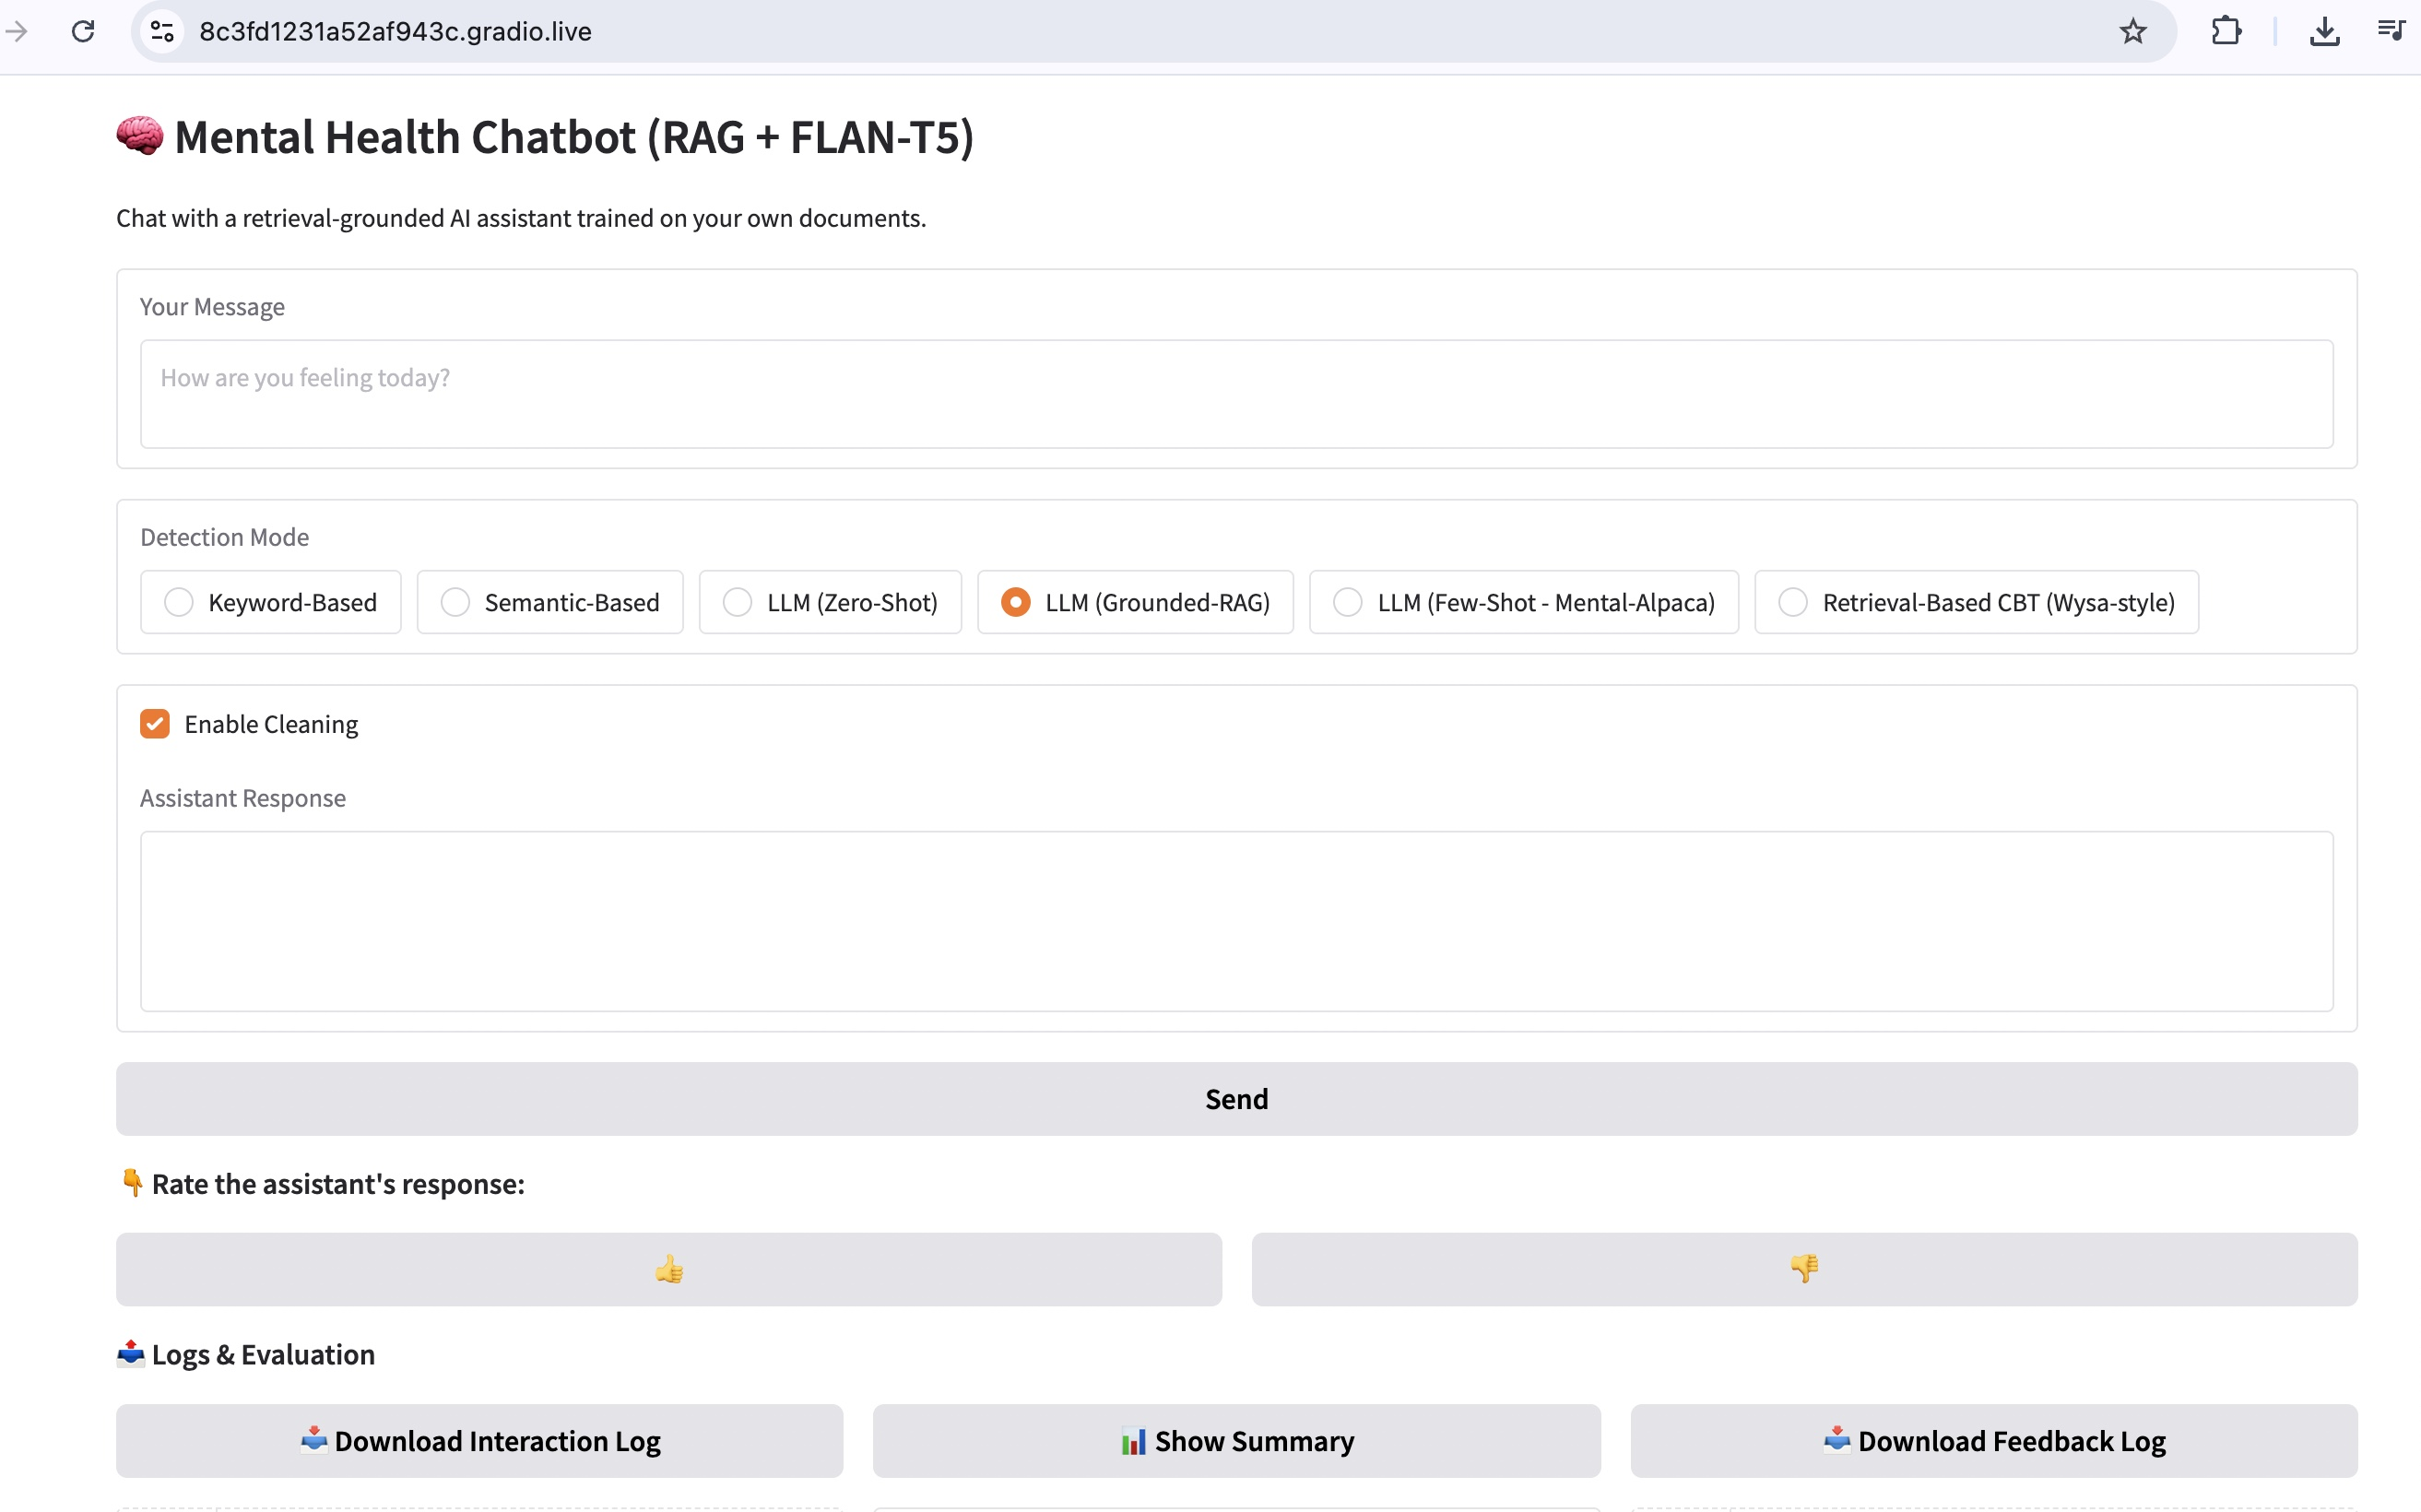
\includegraphics[width=0.8\textwidth]{bot_comparison_tool.jpeg}
    \caption{Comparison tool of Different Types of Mental Health Chatbots}
    \label{fig:bot_comparison}
\end{figure}
We built this comparison to help understand the different types of mental health chatbots described in the literature. By analyzing models like keyword-based bots, semantic-based bots, zero-shot models, grounded models and CBT-based bots, we evaluated their strengths and weaknesses in handling mental health queries. This comparison aligns with the findings from the literature, showcasing how different approaches, from simple keyword matching to complex retrieval-augmented generation and fine-tuned models, offer varying degrees of empathy, accuracy, and context-awareness but the responses offered were questionable in a lot of contexts. 





\subsection{Dataset Impact Comparison} 
This dataset presents a comparative analysis of three chatbot models built upon the GPT-2 base architecture (nsbarla/gpt2-base), each fine-tuned with different training data to explore their responsiveness to emotionally sensitive prompts. One model was trained on a Reddit dataset (nsbarla/gpt2-reddit), another on empathy-rich conversations from Hugging Face (nsbarla/gpt2-empathy) and the third remained as the unaltered baseline. All three models were exposed to the same set of ten distress-related prompts, and their outputs were recorded for comparison. The responses are unique across the models, offering insight into how different training influences affect tone, empathy, and coherence. The empathy-tuned model generally strives to offer supportive or compassionate replies, although some are shallow or lack contextual depth. The Reddit-style model frequently mirrors informal, narrative-driven responses, occasionally incorporating anecdotal elements reflective of real-world user conversations. Conversely, the vanilla model often produces short, vague, or incomplete outputs, indicating limited emotional understanding and generative capacity. Collectively, the dataset reveals distinct stylistic and qualitative differences, shedding light on how training data shapes a model’s ability to engage with sensitive or personal topics.
\begin{table}[H]
    \centering
    \tiny
    \resizebox{\textwidth}{!}{%
    \begin{tabular}{|p{3cm}|p{3cm}|p{3cm}|p{3cm}|}
        \toprule
        \hline
        Prompt & Base Response & Reddit Response & Empathy Response \\
        \hline
        \midrule
        \hline
        I'm feeling really down lately. I don't want to wake up. & I was really & So I'm just going to be taking a shower and eating food. & I am sorry. I hope you can find a new job soon. \\
        \hline
        No one listens to me when I say I'm not okay. & No, I don't care. & No one listens to me when I say I'm not okay. & I'm sorry, I would be so mad at you. \\
        \hline
        I feel like I'm a burden to everyone around me. & I don't want to be on the wrong side of the spectrum. I want to be a person who wants to be respected and respected and respected by all of the other people who don't really understand how I'm supposed to be. I want to be a person who believes in a person who believes in & I feel like I'm an annoying burden to everybody around me. & Oh no \\
        \hline
        I don't know if I can keep going. & I can & I am a social-exchange student and I have a really low self-esteem. & I have a small dog that's just a little bit older. I can't do much about it. \\
        \hline
        I want to feel better, but I can't see a way out. & I want to & I'm doing this because I don't want to be seen as a piece of shit. I just want to be happy. I want to be happy. I want to be happy.  & I was in a housework meeting and saw a big group of people trying to make a sandwich. \\
        \hline
        \bottomrule
    \end{tabular}%
    }
\end{table}


\subsection{Fine-tuned Chatbot with LoRa} 
The Mistral-7B-Instruct-v0.1 model, fine-tuned on a mental health dataset and optimized using LoRA and 4-bit quantization, is now available on Hugging Face under the model ID nsbarla/mental-health-mistral-lora. It was trained on Hugging Face's platform using GPUs, a process that took over 2-3 hours due to the model's size and the applied optimizations. This fine-tuned model is designed to offer more efficient and contextually relevant responses for conversations related to mental health, making it an ideal resource for applications aiming to support users in need of empathetic interactions and advice.
The Mistral Mental Health Bot was trained on a combined dataset consisting of Empathetic Dialogues and Counsel Chat datasets. The Empathetic Dialogues dataset includes conversations designed to encourage empathetic and supportive responses, while the Counsel Chat dataset contains counseling-style dialogues aimed at addressing mental health concerns.
\begin{figure}[h]
    \centering
    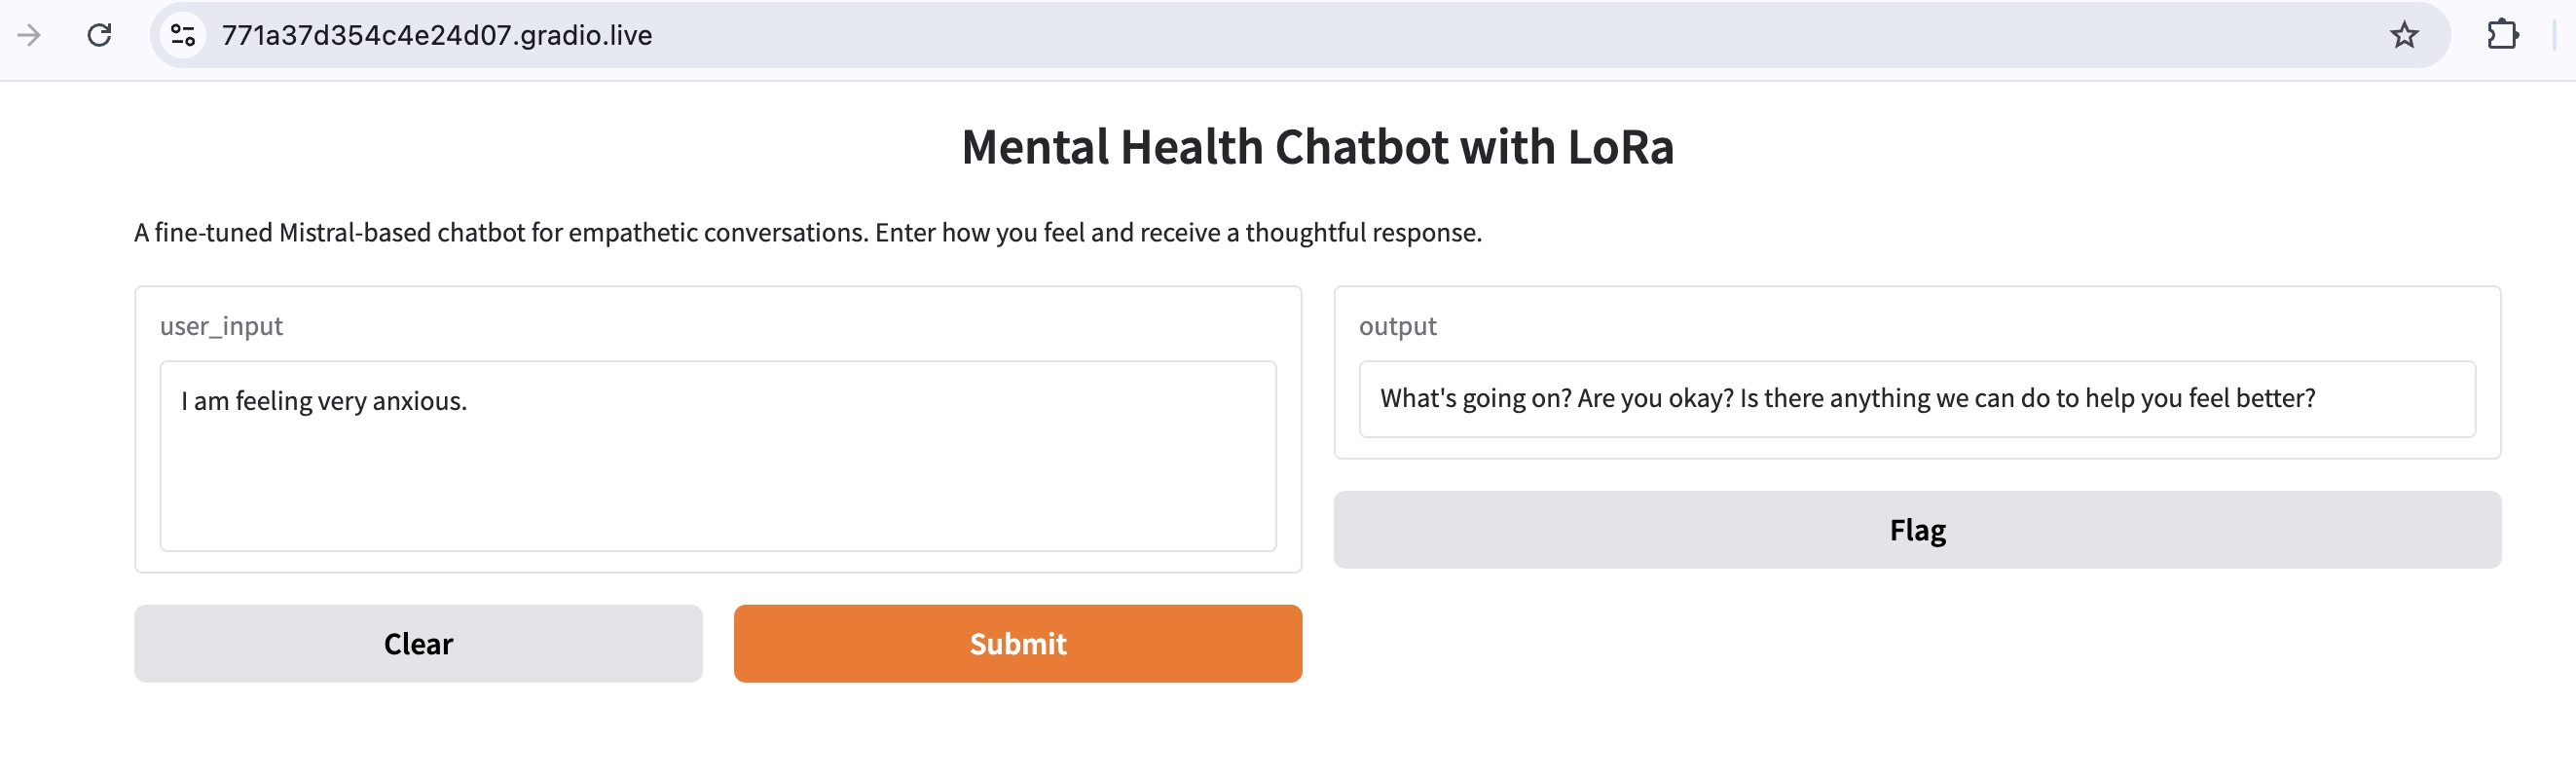
\includegraphics[width=0.8\textwidth]{chatbotwithlora.jpeg}
    \caption{Chatbot with LoRa}
    \label{fig:bot_lora}
\end{figure}
 

\section{Critical Analysis}
    In the development of a mental health chatbot designed to assist individuals experiencing depression, there were several limitations and challenges due to the use of a free platform, the short timeframe of the project (12 weeks), and the complexity of designing an AI-driven tool for such sensitive use cases. This section critically evaluates the chatbot’s performance, highlighting its strengths, limitations, and areas for potential improvement.
\subsection*{Limitations of the Free Platform} 
The decision to use a free platform to build the chatbot imposed significant constraints on its functionality and development. Free platforms typically offer limited resources compared to paid services, which can impact both the scale and quality of the final product. These platforms often restrict access to advanced model features, such as fine-tuning and customisation, and have fewer capabilities for managing large datasets.
For instance, a paid service might provide the ability to train the model on larger and more specific datasets, particularly those related to mental health, which would enhance the chatbot’s ability to provide contextually appropriate and empathetic responses. The limited functionalities of the free platform used in this project prevented the implementation of advanced features such as dynamic backpropagation, which is essential for improving the chatbot’s understanding of context and refining its output over time. Further, the created was built off of a chatbot with generic, and limited training data, meaning that our ability to fine tune this to the required specifications added another layer of complexity.
\subsection*{Data Collection and Model Training Challenges} 
Mental health chatbots require specialized training data that includes therapeutic dialogue, expert-curated mental health advice, and crisis intervention scripts. However, without access to a robust dataset, the chatbot may struggle to provide meaningful and helpful responses. In particular, the chatbot is likely to give generic answers that lack the nuance needed to address the unique experiences of individuals with depression. Furthermore, without fine-tuning the model on mental health-specific data, the chatbot may fail to recognise subtle cues or signs of a more severe mental health crisis, such as suicidal ideation, which could potentially jeopardise the user’s safety.
\subsection*{Ethical and Safety Risks} 
The ethical considerations in developing a mental health chatbot are paramount, especially when the chatbot is intended to engage with vulnerable individuals. In its current form, the chatbot is prone to several ethical risks, particularly around its handling of sensitive topics like suicide and self-harm. A major concern is the chatbot’s tendency to introduce these topics prematurely, even when they have not been mentioned by the user. Such responses can exacerbate distress and disengage users, potentially escalating the situation.
The lack of safety mechanisms in the current model makes it difficult to provide a supportive and responsive environment for users in crisis. In more advanced systems, mechanisms like sentiment analysis, emergency alerts, and crisis detection would allow the chatbot to identify when a user may be in immediate danger and refer them to appropriate resources. Without these safety features, the chatbot’s current use in mental health contexts is problematic, as it may inadvertently cause harm by misinterpreting the user’s emotional state or failing to escalate critical situations when necessary.
\subsection*{Personalisation and Continuity of Care} 
One of the core challenges of the chatbot is its lack of personalisation. Depression is a deeply personal and complex mental health condition, and effective therapeutic tools must be able to adapt to the individual needs of each user. The free platform’s limitations hinder the development of such personalised features, as the chatbot currently struggles to maintain continuity in conversations or respond dynamically to the evolving emotional state of the user.
In a more advanced system, the chatbot would be able to learn from prior interactions with the user, adjusting its tone and responses to better match the user’s emotional context. For example, if the chatbot detects that a user has been expressing consistent feelings of hopelessness or isolation, it could provide more targeted advice or escalate the conversation to a higher level of support. The ability to tailor responses based on the individual’s prior inputs is critical in maintaining user engagement and ensuring the chatbot provides ongoing, meaningful support.
\subsection*{Potential Improvements and Future Directions} 
To enhance the chatbot’s effectiveness, several improvements should be considered in future iterations. Upgrading to a paid platform would allow the chatbot to take advantage of more advanced features, such as model fine-tuning and access to larger, more specialised datasets. With these resources, the chatbot would be able to produce more accurate, contextually relevant, and empathetic responses, particularly in sensitive areas like mental health.
Moreover, to improve the model’s performance, it is essential to collect more diverse and specialised training data. Collaborating with mental health professionals to curate high-quality datasets—such as therapeutic dialogues, expert-curated resources, and crisis intervention scripts—would ensure the chatbot’s responses align with established mental health frameworks. This data would provide the foundation for fine-tuning the model, enabling it to recognise a broader range of emotional cues and handle more complex mental health issues with greater sensitivity.
Additionally, incorporating robust safety features is critical. Future versions of the chatbot should be designed with crisis detection mechanisms that can flag critical emotional states, such as suicidal ideation or severe distress, and trigger appropriate responses. These might include providing emergency contact information or automatically escalating the issue to a mental health professional. Integrating sentiment analysis would further enhance the chatbot’s ability to gauge the emotional tone of conversations, allowing it to respond more sensitively to the user’s state.
Personalisation is another key area for improvement. By allowing the chatbot to track and build upon previous conversations, it could provide more individualised support. The chatbot could adapt its responses based on the user’s unique emotional context and history, offering a more tailored approach to mental health care. This personalised engagement would be crucial in fostering a sense of connection and support, especially for users who may feel isolated or disconnected.
Finally, collaboration with mental health experts throughout the development and fine-tuning stages would ensure that the chatbot adheres to therapeutic guidelines and provides safe, effective support. This input would be invaluable in helping to align the chatbot’s responses with best practices in mental health care, ensuring that it offers both practical advice and compassionate, evidence-based guidance. 

\section{Conclusion}
    \documentclass{article}
\usepackage{lipsum}

\lipsum[7-8] % Example placeholder text. Replace with your actual conclusion. 

\bibliographystyle{apalike}
\bibliography{references}

\appendix
\appendix

\section*{Appendix}
\addcontentsline{toc}{section}{Appendix}

\section{Datasets Used}
\label{appendix:datasets}

We used the following datasets to fine-tune and evaluate the chatbot models.

\begin{itemize}
    \item \textbf{Reddit Dataset 1: Depression Posts (TF-IDF Features)} \\
    A structured dataset containing Reddit posts from depression-related subreddits, with text features pre-processed using TF-IDF vectors. We specifically used the file \texttt{depression\_post\_features\_tfidf\_256.csv} available via Zenodo: \\
    \url{https://zenodo.org/records/3941387}
    
    \item \textbf{Reddit Dataset 2: Suicide Risk Posts} \\
    This dataset includes labeled Reddit posts from 500 users related to suicide risk with annotations, making it useful for identifying emotionally sensitive content. Hugging Face: \\
    \url{https://huggingface.co/datasets/m4faisal/RedditSuicide/commit/5e57cc7e2ebc706b98fbd853a2c52c10b582cd73}
    
    \item \textbf{Empathetic Dialogues Dataset} \\
    A conversational dataset containing 25,000+ short textual dialogues grounded in emotional situations, designed to train models to respond empathetically. Hugging Face: \\
    \url{https://huggingface.co/datasets/facebook/empathetic_dialogues}
\end{itemize}

These datasets were used to fine-tune different variants of the GPT-2 base model, enabling controlled comparisons of style, emotional engagement, and empathy.



\end{document}